%%%%%%%%%%%%%%%%%%%%%%%%%%%%%%%%%%%%%%%%%
% Masters/Doctoral Thesis 
% LaTeX Template
% Version 2.5 (27/8/17)
%
% This template was downloaded from:
% http://www.LaTeXTemplates.com
%
% Version 2.x major modifications by:
% Vel (vel@latextemplates.com)
%
% This template is based on a template by:
% Steve Gunn (http://users.ecs.soton.ac.uk/srg/softwaretools/document/templates/)
% Sunil Patel (http://www.sunilpatel.co.uk/thesis-template/)
%
% Template license:
% CC BY-NC-SA 3.0 (http://creativecommons.org/licenses/by-nc-sa/3.0/)
%
%%%%%%%%%%%%%%%%%%%%%%%%%%%%%%%%%%%%%%%%%

%-----------------
%	PACKAGES AND OTHER DOCUMENT CONFIGURATIONS
%-----------------

\documentclass[
11pt, % The default document font size, options: 10pt, 11pt, 12pt
%oneside, % Two side (alternating margins) for binding by default, uncomment to switch to one side
english, % ngerman for German
onehalfspacing, % singlespacing Single line spacing, alternatives: onehalfspacing or doublespacing
%draft, % Uncomment to enable draft mode (no pictures, no links, overfull hboxes indicated)
%nolistspacing, % If the document is onehalfspacing or doublespacing, uncomment this to set spacing in lists to single
liststotoc, % Uncomment to add the list of figures/tables/etc to the table of contents
toctotoc, % Uncomment to add the main table of contents to the table of contents
%parskip, % Uncomment to add space between paragraphs
nohyperref, % Uncomment to not load the hyperref package
headsepline, % Uncomment to get a line under the header
%chapterinoneline, % Uncomment to place the chapter title next to the number on one line
%consistentlayout, % Uncomment to change the layout of the declaration, abstract and acknowledgements pages to match the default layout
]{MastersDoctoralThesis} % The class file specifying the document structure

\usepackage[utf8]{inputenc} % Required for inputting international characters
\usepackage[T1]{fontenc} % Output font encoding for international characters

\usepackage{mathpazo} % Use the Palatino font by default

\usepackage[backend=bibtex,style=numeric,natbib=true, sorting=none]{biblatex} % Use the bibtex backend with the authoryear citation style (which resembles APA)

\addbibresource{example.bib} % The filename of the bibliography

\usepackage[autostyle=true]{csquotes} % Required to generate language-dependent quotes in the bibliography

\usepackage{arabxetex}

\usepackage[printonlyused,withpage]{acronym}

\usepackage{algorithmic}


%-----------------
%	MARGIN SETTINGS
%-----------------

\geometry{
	paper=a4paper, % Change to letterpaper for US letter
	inner=2.5cm, % Inner margin
	outer=3.8cm, % Outer margin
	bindingoffset=.5cm, % Binding offset
	top=1.5cm, % Top margin
	bottom=1.5cm, % Bottom margin
	%showframe, % Uncomment to show how the type block is set on the page
}

%-----------------
%	THESIS INFORMATION
%-----------------

\thesistitle{Thesis Title} % Your thesis title, this is used in the title and abstract, print it elsewhere with \ttitle
\supervisor{Dr. James \textsc{Smith}} % Your supervisor's name, this is used in the title page, print it elsewhere with \supname
\examiner{} % Your examiner's name, this is not currently used anywhere in the template, print it elsewhere with \examname
\degree{Doctor of Philosophy} % Your degree name, this is used in the title page and abstract, print it elsewhere with \degreename
\author{John \textsc{Smith}} % Your name, this is used in the title page and abstract, print it elsewhere with \authorname
\addresses{} % Your address, this is not currently used anywhere in the template, print it elsewhere with \addressname

\subject{Biological Sciences} % Your subject area, this is not currently used anywhere in the template, print it elsewhere with \subjectname
\keywords{} % Keywords for your thesis, this is not currently used anywhere in the template, print it elsewhere with \keywordnames
\university{University Name} % Your university's name and URL, this is used in the title page and abstract, print it elsewhere with \univname
\department{Department or School Name} % Your department's name and URL, this is used in the title page and abstract, print it elsewhere with \deptname
\group{Research Group Name} % Your research group's name and URL, this is used in the title page, print it elsewhere with \groupname
\faculty{Faculty Name} % Your faculty's name and URL, this is used in the title page and abstract, print it elsewhere with \facname

% \AtBeginDocument{
% \hypersetup{pdftitle=\ttitle} % Set the PDF's title to your title
% \hypersetup{pdfauthor=\authorname} % Set the PDF's author to your name
% \hypersetup{pdfkeywords=\keywordnames} % Set the PDF's keywords to your keywords
% }

\begin{document}


\frontmatter % Use roman page numbering style (i, ii, iii, iv...) for the pre-content pages

\pagestyle{plain} % Default to the plain heading style until the thesis style is called for the body content

%-----------------
%	TITLE PAGE
%-----------------

\begin{titlepage}
\begin{center}

\vspace*{.06\textheight}
{\scshape\LARGE \univname\par}\vspace{1.5cm} % University name
\textsc{\Large Doctoral Thesis}\\[0.5cm] % Thesis type

\HRule \\[0.4cm] % Horizontal line
{\huge \bfseries \ttitle\par}\vspace{0.4cm} % Thesis title
\HRule \\[1.5cm] % Horizontal line
 
\begin{minipage}[t]{0.4\textwidth}
\begin{flushleft} \large
\emph{Author:}\\
\authorname % Author name - remove the \href bracket to remove the link
\end{flushleft}
\end{minipage}
\begin{minipage}[t]{0.4\textwidth}
\begin{flushright} \large
\emph{Supervisor:} \\
\supname % Supervisor name - remove the \href bracket to remove the link  
\end{flushright}
\end{minipage}\\[3cm]
 
\vfill

\large \textit{A thesis submitted in fulfillment of the requirements\\ for the degree of \degreename}\\[0.3cm] % University requirement text
\textit{in the}\\[0.4cm]
\groupname\\\deptname\\[2cm] % Research group name and department name
 
\vfill

{\large \today}\\[4cm] % Date
%\includegraphics{Logo} % University/department logo - uncomment to place it
 
\vfill
\end{center}
\end{titlepage}

%------------------
%	DECLARATION PAGE
%--------------------

% \begin{declaration}
% \addchaptertocentry{\authorshipname} % Add the declaration to the table of contents
% \noindent I, \authorname, declare that this thesis titled, \enquote{\ttitle} and the work presented in it are my own. I confirm that:

% \begin{itemize} 
% \item This work was done wholly or mainly while in candidature for a research degree at this University.
% \item Where any part of this thesis has previously been submitted for a degree or any other qualification at this University or any other institution, this has been clearly stated.
% \item Where I have consulted the published work of others, this is always clearly attributed.
% \item Where I have quoted from the work of others, the source is always given. With the exception of such quotations, this thesis is entirely my own work.
% \item I have acknowledged all main sources of help.
% \item Where the thesis is based on work done by myself jointly with others, I have made clear exactly what was done by others and what I have contributed myself.\\
% \end{itemize}
 
% \noindent Signed:\\
% \rule[0.5em]{25em}{0.5pt} % This prints a line for the signature
 
% \noindent Date:\\
% \rule[0.5em]{25em}{0.5pt} % This prints a line to write the date
% \end{declaration}

% \cleardoublepage

%-----------------
%	QUOTATION PAGE
%-----------------

% \vspace*{0.2\textheight}

% \noindent\enquote{\itshape Thanks to my solid academic training, today I can write hundreds of words on virtually any topic without possessing a shred of information, which is how I got a good job in journalism.}\bigbreak

% \hfill Dave Barry

%-----------------
%	ABSTRACT PAGE
%-----------------

\begin{abstract}
\addchaptertocentry{\abstractname} % Add the abstract to the table of contents
The Thesis Abstract is written here (and usually kept to just this page). The page is kept centered vertically so can expand into the blank space above the title too\ldots
\end{abstract}

%-----------------
%	ACKNOWLEDGEMENTS
%-----------------

\begin{acknowledgements}
\addchaptertocentry{\acknowledgementname} % Add the acknowledgements to the table of contents
The acknowledgments and the people to thank go here, don't forget to include your project advisor\ldots
\end{acknowledgements}

%-----------------
%	LIST OF CONTENTS/FIGURES/TABLES PAGES
%-----------------

\tableofcontents % Prints the main table of contents

\listoffigures % Prints the list of figures

\listoftables % Prints the list of tables

%-----------------
%	ABBREVIATIONS
%-----------------

\begin{abbreviations}{ll} % Include a list of abbreviations (a table of two columns)

% \textbf{LAH} & \textbf{L}ist \textbf{A}bbreviations \textbf{H}ere\\
% \textbf{WSF} & \textbf{W}hat (it) \textbf{S}tands \textbf{F}or\\

\end{abbreviations}
\begin{acronym}
	\acro{USA}{Uited States of America}
\end{acronym} 

%-----------------
%	PHYSICAL CONSTANTS/OTHER DEFINITIONS
%-----------------

% \begin{constants}{lr@{${}={}$}l} % The list of physical constants is a three column table

% % The \SI{}{} command is provided by the siunitx package, see its documentation for instructions on how to use it

% Speed of Light & $c_{0}$ & \SI{2.99792458e8}{\meter\per\second} (exact)\\
% %Constant Name & $Symbol$ & $Constant Value$ with units\\

% \end{constants}

%-----------------
%	SYMBOLS
%-----------------

% \begin{symbols}{lll} % Include a list of Symbols (a three column table)

% $a$ & distance & \si{\meter} \\
% $P$ & power & \si{\watt} (\si{\joule\per\second}) \\
% %Symbol & Name & Unit \\

% \addlinespace % Gap to separate the Roman symbols from the Greek

% $\omega$ & angular frequency & \si{\radian} \\

% \end{symbols}

%-----------------
%	DEDICATION
%-----------------

\dedicatory{For/Dedicated to/To my\ldots} 



%-----------------
%	THESIS CONTENT - CHAPTERS
%--------------------

\mainmatter % Begin numeric (1,2,3...) page numbering

\pagestyle{thesis} % Return the page headers back to the "thesis" style

   
% Include the chapters of the thesis as separate files from the Chapters folder
% Uncomment the lines as you write the chapters

% Chapter Template

\chapter{Introduction} % Main chapter title

\label{chp:intro} % Change X to a consecutive number; for referencing this chapter elsewhere, use \ref{ChapterX}

% Chapter Template

\chapter{Background} % Main chapter title

\label{ChapterX} % Change X to a consecutive number; for referencing this chapter elsewhere, use \ref{ChapterX}
Batch normalization algorithm is described as follows:



\vspace*{1.3\baselineskip}
\begin{algorithmic}[1]

\REQUIRE : Minibatch activation values $x$ : $\mathcal B = \{x_{1,\ldots,m}\}$ ; parameters to be learned $\gamma$ ,$\beta$.

\ENSURE  : $\{y_i = \mathrm{BN}_{\gamma,\beta}(x_i)\}$
\vspace*{.7\baselineskip}
\STATE $\mu_{\mathcal B} \leftarrow \frac1m \sum_{i = 1}^m x_i$
\vspace*{.7\baselineskip}
\STATE $\sigma^2_{\mathcal B} \leftarrow \frac1m \sum_{i=1}^m (x_i - \mu_{\mathcal B})^2$
\vspace*{.7\baselineskip}
\STATE $\hat x_i \leftarrow \frac{x_i - \mu_{\mathcal B}}{\sqrt{\sigma_{\mathcal B}^2 + \epsilon}}$
\vspace*{.7\baselineskip}
\STATE $y_i \leftarrow \gamma \hat x_i + \beta \equiv \mathrm{BN}_{\gamma,\beta}(x_i)$

\end{algorithmic} 
% Chapter Template

\chapter{Literature Review} % Main chapter title

\label{chp:related} % Change X to a consecutive number; for referencing this chapter elsewhere, use \ref{ChapterX}

Convolutional Neural Network (CNN) outperformed traditional computer vision approaches for medical image classification due to its current advances on architecture design. Typically, CNN architectures are composed of two parts~\cite{krizhevsky2012imagenet}. First part is called a convolutional part which further consists of  convolutional layers interconnected with some connection patterns that are responsible for feature extraction. Second part is the fully connected layers which consist of Dense layers that are responsible for classification. This section discusses previous CNN based CXR classification systems  reporting the modeling mechanisms and the reported results.
\section{CNN Based Models}
In this section CNN base models for covid detection is reviewed.
\subsection{Reliable COVID-19 Detection Using Chest X-ray Images}
\begin{figure}
    \begin{center}
        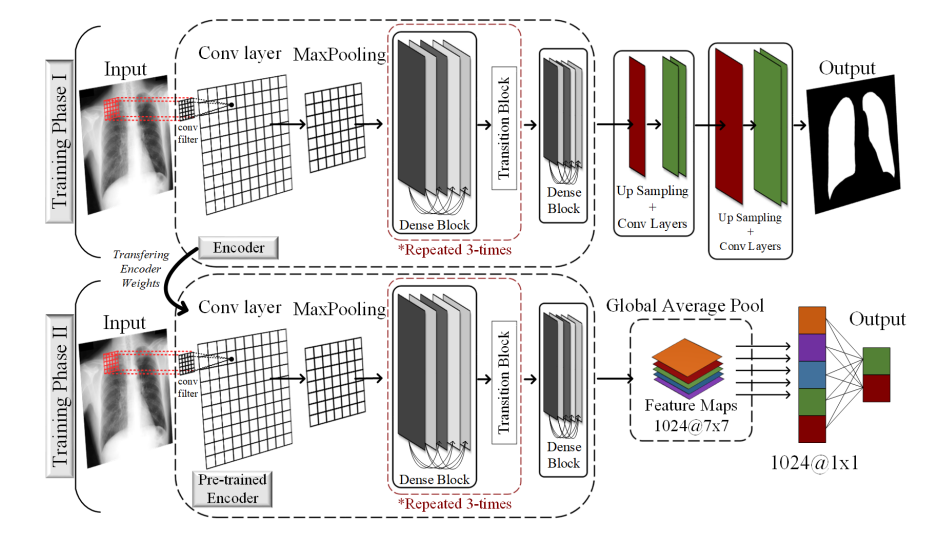
\includegraphics[width=\textwidth]{Figures/RltDag.png}
        \caption{\label{rlt:dag} ReCovNet model proposed by~\cite{dag}. It uses pretrained encoder for classification of COVID-19 CXR image}
    \end{center}
\end{figure}
In \cite{dag}, authors have adapted transfer learning techniques to train CNN models. Training is performed through two phases. Fig.~\ref{rlt:dag} represent proposed system by \cite{dag}. In phase I, u-shaped architecture is excluded by removing the skip connections, which performs the concatenation operation. The reason for constructing an encoder-decoder network without skip connections is that the contributions from the initial layers are avoided; therefore, the network can make decisions from the high level features that are closer to segmentation mapping of the input image.  In phase II, Decoder network is discarded, and the encoder network is fine-tuned for the binary classification task. Adam optimizer is used to train their network. Model is trained with QaTa-COV19 dataset. The method achieved a performance of 98.57\% for sensitivity and 99.77\%  for specificity.

\subsection{Advance Warning Methodologies for
COVID-19 Using Chest X-Ray Images}

% In \cite{ar}, authors have proposed Convolutional Support Estimator Networks (CSENs) classifier. CSEN is used to classify features extracted by DenseNet-121. DenseNet-121 is pre-trained using ImageNet Dataset then fine-tuned using QaTa-Cov19. CSEN achieved 97\% of sensitivity and over 95.5\% of specificity. Authors also evaluated DenseNet-121 achieving 95\% of  sensitivity and 99.74\% of specificity.

In \cite{ar}, authors evaluated the performance of different classifier for classifying the feature produced by DenseNet121. Their methedology is as follows:
\subsubsection{Feature Extraction using DensNet121}
They pretrained two DenseNet121~\cite{huang2017densely} models on Early-QaTa-COV19 and ChestX-ray14 datasets are used to extract 1024-D feature vectors by taking the output after global pooling just before the classification layer. Then, a dimensionality reduction is applied over the calculated features with principal component analysis (PCA) by choosing the first $512$ principal components.

\subsubsection{Representation-based classification}
 Representation-based classification (RC) techniques are used in many different classification tasks such as face recognition in~\cite{wright2010sparse}, hyperspectral image classification~\cite{li2016survey}, and human action recognition~\cite{guha2011learning}. Authors classified the feature vector produced by DenseNet121 using either Sparse RC or Collaborative RC. It is performed as follows:
 \begin{equation}
    \begin{split}
        \hat{x} = \arg \min_{x}(\lambda \vert \vert x \vert\vert_{1} + \vert\vert y - Dx \vert\vert_{2})
    \end{split}
\end{equation}
where $D$ is the dictionary of feature produced by DenseNet121 and projected using PCA. Sparse RC minimizes $\ell^{1}$ of $\hat{x}$. While Collaborative RC minimizes $\ell^{2}$ of $\hat{x}$ as follows:
\begin{equation}
    \begin{split}
        \hat{x} = \arg \min_{x}(\lambda \vert \vert x \vert\vert_{2} + \vert\vert y - Dx \vert\vert_{2})
    \end{split}
\end{equation}
For both types of representations $\hat{x}$ reconstruction error is calculated as follows:
\begin{equation}
    \begin{split}
        e_i = \vert\vert y - D\hat{x} \vert\vert_2
    \end{split}
\end{equation}
Then assign a class of the lower construction error as follows:
\begin{equation}
    \begin{split}
        class(y) \arg \min(e_i)
    \end{split}
\end{equation}

Fig.~\ref{fig:RC} represent representation classification pipeline presented in~\cite{ar}. They achieved a $.98$ and $.97$ of accuracy for Sparse Representation-based classification and Collaborative Representation-based classification, respectively. 
\begin{figure}
    \centering
    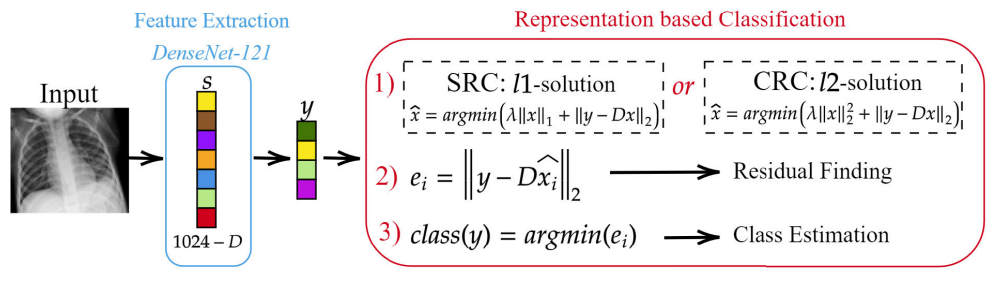
\includegraphics[width=\textwidth]{Figures/RCpipline.png}
    \caption{\label{fig:RC} sparse and Collaborative Representation learning pipeline of~\cite{ar}}
\end{figure}
Authors of~\cite{ar} also evaluated SVM for classifying features produces by DenseNet121 and recorded $.98$ of accuarcy.



%  \begin{algorithm}[H]
%     \DontPrintSemicolon
%     \caption{Sparse Representation-based Classification (SRC)}
%     \KwIn{a matrix of training samples $A = [A_{1}, A_{2}, \dots ,A_{k}] \in \mathbb{R}^{m \times n}$ 
%       for $k$ classes, a test sample $\mathbf{y} \in \mathbb{R}^{m}$, (and an optional error tolerance $\varepsilon > 0$).}
  
%     Normalize the columns of $A$ to have unit $\ell^{2}$-norm.\;
%     Solve the $\ell^{1}$-minimization problem:
%     $\hat{\bm{x}}_{1} = \arg \min_{x}\norm{\bm{x}}_{1}\quad \text{subject to}\quad A\bm{x} = \bm{y}$ \;
%     (Or alternatively, solve
%     $\hat{\bm{x}}_{1} = \arg \min_{x}\norm{\bm{x}}_{1}\quad \text{subject to}\quad \norm{A\bm{x} = \bm{y}}_{2} \leqslant \varepsilon$).\;
%     Compute the residuals $r_{i}(\bm{y}) = \norm{\bm{y} - A \delta_{i}(\hat{\bm{x}}_{1})}_{2}$\;
%     \For{$i = 1,\dots,k$}{something}
%   \end{algorithm}
  
\section{COVID-19 Detection Using DL Algorithm on CXR Images}

In \cite{akt}, authors proposed a modified MobileNetV2 CNN model where the stander convolution is replaced by a depth-wise convolution. Their model is trained with $3616$ COVID-19 CXR images and 10,192 normal CXR images. Dataset is initially preprocessed by reshaping input images to $299\times299$ and image enhancement technique is applied. The model achieved a accuracy of 98\% for binary classification task.

In \cite{acos}, authors proposed a two phase COVID-19 multi-label classification system. The system phase I classifies the input CXR images as normal or COVID-19. In case the image  is classified as COVID-19, phase II further classifies this image as pneumonia or COVID-19. Phase I and Phase II have the same structure with a total of $8196$  local features are extracted then classified using ensemble module. Base classifier of the ensemble module consist of NB, ANN, DT and SVM. A majority voting is used to combine the predictions of these classifiers. Their system achieved accuracy of $98.062$\%  and $91.329$\% for Phase I and Phase II, respectively.\\
In \cite{hyp} authors have proposed a hybrid model for multilabel classification where VGG16 is used as a feature extractor. Their system is trained by a combined dataset of QaTaCov19 and Chest X-Ray achieving accuracy of $91.09$\%.

Despite the high accuracy of current CNN based CXR classification methods, but these methods don't address the problem that CNN is scale variant model. This problem hinders the recognition of large scale COVID-19 pneumonia. In this paper, a novel scale-invariant CNN architecture is proposed for classification of COVID-19 pneumonia. The proposed architecture deploys Atrous convolution method for learning the scale-invariant features. Then, an attention model is utilized to automatically and internally select at which scale  CNN should consider and ignore other scales. The proposed architecture exploits texture augmentation to reduce the overfitting and artificially enlarge the training dataset. The experimental results show that proposed system outperforms  the previous  CNN based CXR classification methods  with lower trainable parameter number.


\begin{table}[htbp]
\caption{\label{tbl:related}Overview of recent studies for classifying COVID19}
\begin{center}
\begin{adjustbox}{angle=90}
\begin{tabular}{|l|r|r|l|l|l|}%{lrrlll}
\hline
Work &  \#Samples &  Classes &  Model &  Best Performing Model &   Performance \\
\hline
\hline
~\cite{35apostolopoulos2020covid} & 1428 &    3 & VGG19, MobileNetV2, &   MobileNetV2 & Acc = 96.78\%  \\

      &      &    & Inception, Xception &    &   \\
\hline
~\cite{36hall2020finding} &  204 &    2 &   VGG16 + Resnet50 & VGG16 + Resnet50, &    Acc = 89.2\% \\

     &    &      &                        &   custom CNN &      \\
\hline           
~\cite{37narin2021automatic} &  100 &    2 &   ResNet50, InceptionV3, &  ResNet50 &  Acc = 98\% \\

&    &      &   and InceptionRes-NetV2 &   &    \\
\hline
~\cite{38tang2020automated} &    21152 &    2 &    CNN &   CNN &   Acc = 94.64\% \\
\hline
~\cite{39minaee2020deep}  & 5184 &    2 &   ResNet18, ResNet50, &    SqueezeNet & Sensitivity = 98\%\\

  &   &      &     SqueezeNet, DenseNet-121 &      &  \\
\hline
~\cite{40afshar2020covid}  &    13975 &    2 & COVID-CAPS &    COVID-CAPS &   Acc = 95.7\%, \\
\hline
~\cite{41ahsan2020covid}  &  400 &    2 & VGG16, InceptionResNetV2, &  NasNetMobile &   Acc = 93.94\% \\

  &    &      &  ResNet50, DenseNet201  &    &     \\
\hline
~\cite{42hemdan2020covidx}  &   75 &    2 & VGG19, Xception,  &   VGG19, DenseNet &   F1 scores = 0.91 \\

  &     &      &  ResNetV2, DenseNet201 &     &    \\
\hline
~\cite{43ozturk2020automated}  & 1127 &    2 &   Modified Darknet &  Modified Darknet &  Acc = 98\% \\
\hline
~\cite{44khan2020coronet}  & 1257 &    3 &   Xception &  Xception &  Acc = 94\% \\
\hline
~\cite{45chandra2021coronavirus} & 2356 &    3 &    ACoS system &  ACoS &   Acc = 91.33\% \\
\hline
~\cite{46sekeroglu2020covid19} & 6100 &    3 & SVM, LR, DT, &   Mean result &    Acc = 98.5\% \\

  &   &      &   kNN + VGG16,  &    &    \\

  &   &      &    ResNet50 &    &    \\
\hline
~\cite{47pandit2021automatic}& 1428 &    2 &  VGG16 & VGG16 &  Acc = 96\% \\
\hline
~\cite{48arias2020artificial} &    79500 &    3 &   Grad-CAM &  Grad-CAM &    Acc = 91.5\% \\
\hline
~\cite{49yamac2021convolutional} & 6200 &    4 &  CSEN-based classifier & CSEN-based Classifier &    Sensitivity = 98\% \\
\hline
~\cite{50wang2020covid} &    13975 &   19 &  COVID-Net & COVID-Net &    Acc = 93.3\% \\
\hline
~\cite{51abbas2021classification} &  196 &    3 & DeTrac &    Detrac &    Acc = 93.1\% \\
\hline
~\cite{52toraman2020convolutional} & 3150 &    3 &    CapsNet &   CapsNet &  Acc = 97\% \\
\hline
~\cite{53das2022automated} & 1127 &    3 &   Xception &  Xception &  Acc = 97\% \\
\hline
~\cite{54hu2020learning} & 7470 &    2 &    MD-Conv &   MD-Conv &    Acc = 93.4\% \\
\hline
~\cite{55ismael2021deep} &  380 &    2 &    Novel CNN Model &   Novel CNN Model &    Acc = 91.6\% \\
\hline
~\cite{56shankar2021optimal} &  247 &    2 &   BMO-CRNN &  BMO-CRNN &  Acc = 97.31\% \\
\hline
\end{tabular}
\end{adjustbox}
\end{center}
\end{table}


% Chapter Template

\chapter{Proposed Methodologies} % Main chapter title

\label{chp:proposed1} % Change X to a consecutive number; for referencing this chapter elsewhere, use~\ref{ChapterX}
In this chapter, a novel architecture is introduced for detecting COVID-19 that is designed to be lightweight. The architecture is based on two key components: spatial kernel separability and residual connection. By exploiting spatial kernel separability, the number of training parameters is significantly reduced, making the model more computationally efficient. Additionally, residual connections are used extensively to maintain network stability during the training process and to provide the model with regularization effects that reduce overfitting. This combination of spatial kernel separability and residual connections creates a lightweight architecture that is highly effective at detecting COVID-19. Overall, this chapter provides a valuable contribution to the field of COVID-19 detection by introducing a novel and efficient architecture that can help to identify the disease quickly and accurately. 

\begin{figure}[th]
    \centering
    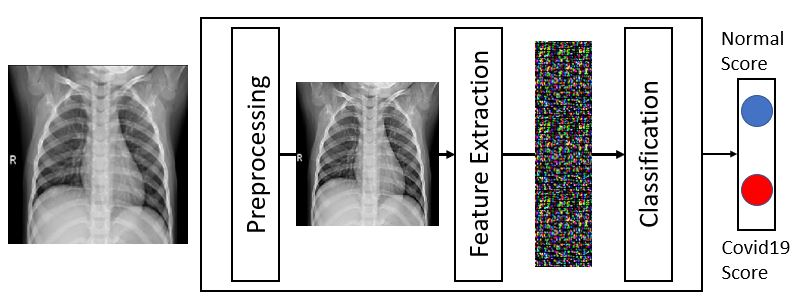
\includegraphics[height=40mm,width=8.0cm]{Figures/fig1.jpg}
    % \decoRule
    \caption{The phases of the proposed method I.}
    \label{fig1}
    \end{figure}

\section{Methodology I}
In this section, a  proposed method I to detect COVID-19 disease from chest X-ray images is presented. The proposed method exploits the CNN model to classify the input chest X-ray image into one of two categories; normal case or Covid-19 case. The proposed method I consists of three phases: preprocessing, feature extraction, and classification. The proposed method phases are shown in Fig.~\ref{fig1}. 

\subsection{Preprocessing Phase}

The preprocessing phase is responsible for resizing and normalizing the input chest X-ray images. The pre-processing phase is employed to maintain the numerical stability of the model and reduce the co-variance shift~\cite{lecun1989handwritten}. In addition, this phase leads the learning model of the CNN model to reduce the required overhead to adapt to the different scales of different features of the input data. Reshaping size is determined empirically. The input chest X-ray image is re-sized and then adapted and normalized to a normal distribution as follows:

\begin{equation}
Y := \frac{x_i - \mu_{\mathcal B}}{\sqrt{\sigma_{\mathcal B}^2 + \epsilon}}
\label{eq1}
\end{equation}
where $\mu$ and $\sigma$ are the mean and standard deviation of chest X-ray image (X), respectively.

After re-sizing the input chest X-ray image, the input image is normalized to have a zero mean and unit standard deviation. Then,  the image can be scaled and shifted with a normalization parameter which is determined and adapted by the training dataset during the training process according to the following equation: 

\begin{equation}
Z := w_1 Y + w_2
\label{eq2}
\end{equation}
where $w_1$ and $w_2$ are a trainable parameter.

Unlike the normalization method presented in~\cite{ioffe2015batch}, the batch normalization process presented in this paper has a $z$-score normalization parameter that is used in both the training and validation phases.


\subsection{Feature Extraction and Classification}

CNN models achieved outstanding success in image recognition~\cite{lecun2015deep}. This phase is responsible for extracting spatial features from the normalized chest X-ray image using a tailored CNN model.  This phase is based on learning the CNN model by the input preprocessed chest X-ray images. The design of the tailored CNN model is described as follows: 

\subsubsection{Separable CNN kernels}
\begin{figure*}
\begin{center}
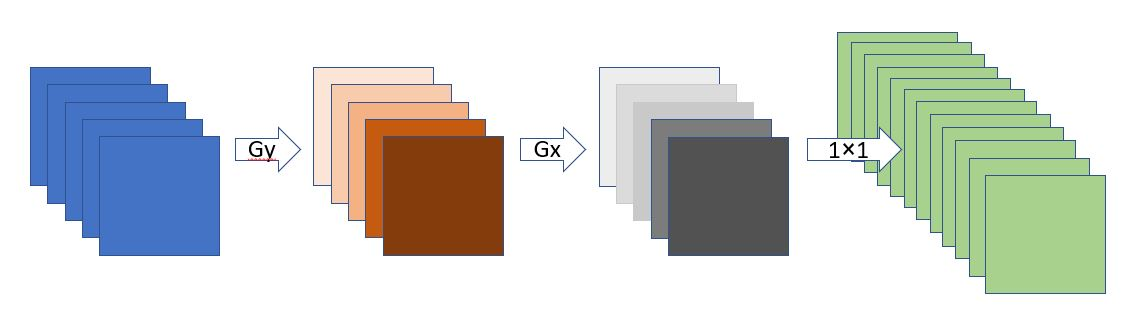
\includegraphics[height=33mm,width=14.0cm]{Figures/fig2.jpg}
\caption{Separable convolution  $Gy$ and $Gx$ have kernel size of $M\times1$ and $1 \times M$. The combination of these kernels is approximately a $M\times M$ kernel and depth-wise convolution is applied by a $1\times1$ convolution. The output depth is padded with zeros to have the same spatial size of  $Gy, Gx$. $Gy, Gx$ are performed channel-wise. }
\label{fig2}\end{center}\end{figure*}


    
Kernel separability~\cite{rigamonti2013learning}~\cite{szegedy2017inception} is based on decomposing a 2D convolution kernel to linear combinations of two 1D vectors which leads to a large reduction in the total number of resulting parameters. For example, a 2D kernel of size $9 \times 9$ has a total number of $9^2 = 81$  trained parameters. Whereas in the case of separating this 2D kernel to linear combinations of two 1D vectors of sizes $9 \times 1$ and $1 \times 9$, this results in a total number of  $9 + 9 = 18$ trained parameters. As a consequence, kernel separability reduces the number of CNN model operations (such as multiplication and addition). A  2D kernel of $k \times k$ applied for a 2D signal with spatial dimensions of $ M \times N$ has a total number of  $(N-4)(M-4)\times k^2$ operations but in case of applying kernel separability yields $2(N-4)(M-4)k$ operations. The flow of separated convolution operation is summarized in Fig.~\ref{fig2}. Fig.~\ref{fig3} represents the structure, denoted by the Separated Convolutional Layer, used in the proposed method with kernel size of $(M\times N)$ and satisfying the convolutional kernel separability. Separated Convolutional Layer is composed of three consecutive layers. The first convolutional layer has a kernel size of $(M\times1)$ and the number of convolutional neurons and filters are equal to the number of channels as the input feature map and the convolution operations are performed channel-wise. The second layer operates in the same way as the first layer but it has a kernel of size $(1\times M)$. The third layer is the convolutional layer with a kernel of size $(1\times1)$ and the number of convolutional neurons is $N$. The collaboration of the three layers are connected to perform similarly to the convolutional layer with a kernel size of $(M\times M)$ and the number of neuron and filter is the same as $N$ but with a large difference in the performance.


\begin{figure}
    \begin{center}
    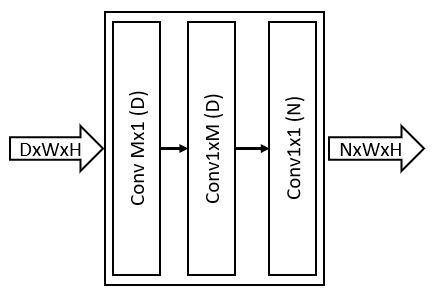
\includegraphics[height=34mm,width=7.0cm]{Figures/fig3.jpg}
    \caption{Separated Convolutional Layer}{ composed of three consecutive layers. The first Convolutional layer has a kernel size of $(M\times1)$ and $D$  convolutional neuron. The second layer operates in the same way as the first layer but it has a kernel of size $(1\times M)$ and $D$ convolutional neuron. The third layer is the convolutional layer with a kernel of size $(1\times1)$ and the number of convolutional neurons is $N$.}
    \label{fig3}
    \end{center}
    \end{figure}

\subsubsection{ Batch Normalization and  Activation function}

In the proposed method linear separable convolutional kernels are followed by a batch normalization and an activation function. Rectified Linear Unit (ReLU)~\cite{he2015delving} is a nonlinear activation that allows the network to fit and approximate highly non-linear dataset distribution. The proposed method employs batch normalization which is described in~\cite{ioffe2015batch}. 

Batch Normalization~\cite{ioffe2015batch} reduces internal covariate shift produced as a result of moving between layers during the feedforward procedure~\cite{ioffe2015batch}. Batch Normalization makes the loss landscape smoother and reduces the number of saddle points~\cite{santurkar2018does} which allows to use of higher learning rates. Using a higher learning rate makes the network training  faster~\cite{ioffe2015batch}. Batch normalization reduces the vanishing gradient problem and exploding gradient problem as it makes the resulted activation scale independent from the trainable parameter scale~\cite{ioffe2015batch}. Batch normalization has the effect of regularization because of the inherited randomness when selecting the batch sample~\cite{ioffe2015batch} which help the generalization to unseen chest X-ray image.

\subsubsection{ Deep and larger receptive field Network design}

Deeper convolutional neural network design is a very important task for any image recognition task~\cite{he2016deep}. Training a deeper network is very expensive and has many challenges such as vanishing gradient problem, exploding gradient problem, and degradation problem~\cite{he2016deep}. The exploding gradient problem occurs when the gradient update becomes very large (approaching infinity) resulting in the network diversion. A vanishing gradient problem occurs when the gradient update becomes very small (approaching zero) resulting in preventing the parameter update for early layers~\cite{ioffe2015batch} and preventing the network from learning new patterns. Batch normalization~\cite{ioffe2015batch} and the use of ReLU activation function~\cite{krizhevsky2012imagenet} alleviate these two problems.

The deep layers of CNN networks sometimes need to approximate the identity function which is not a simple task, especially with the existence of a non-linear function. Residual connection~\cite{he2016deep} overcomes this problem by using skip connection as shown in Fig.~\ref{fig4}.
Fig.~\ref{fig4} represents the building block layer of the feature extraction phase, denoted by a stack of Residual Separated Block  (RSB). RSB consists of four layers of separated convolutional layers, each layer is followed by a batch normalization and an activation function. It has an output of depth $N$ where each sublayer produces an output of depth $N/4$ which is concatenated at the end of the layer to produce a depth  $N$. RSB produces a feature map that includes both low-level features and high-level features.

\begin{figure*}
\begin{center}
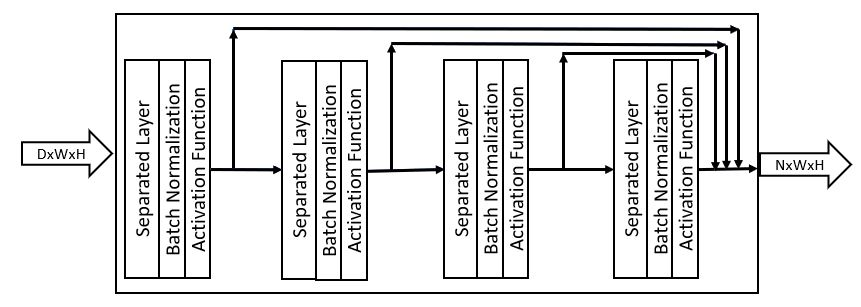
\includegraphics[height=38mm,width=14.0cm]{Figures/fig4.jpg}
\caption{The stack of residual separated block  (RSB) consists of four layers of separated convolutional layer each of which is followed by batch normalization and activation function. Feature maps are concatenated at the end of the block.}
\label{fig4}
\end{center}
\end{figure*}

\begin{figure*}
    \begin{center}
    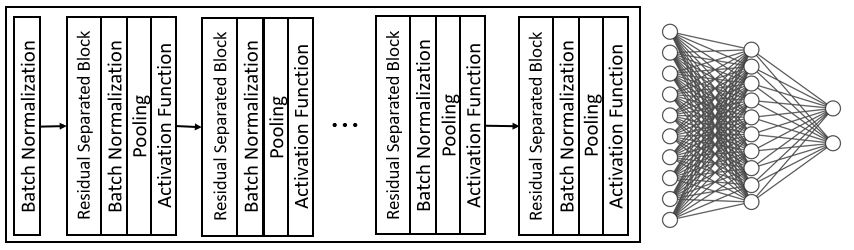
\includegraphics[height=37mm,width=14.0cm]{Figures/fig5.jpg}
    \caption{The complete proposed tailored CNN architecture.}
    \label{fig5}
    \end{center}
    \end{figure*}
    
Unlike the traditional neural network, which is fully connected to the previous layer, the convolutional neural network is connected locally to a local region of the previous feature map. This introduces the concept of the network receptive field~\cite{luo2016understanding}. The receptive field should be large enough to capture large patterns in the input chest X-ray image. Therefore, any consecutive convolutional layers in the proposed method without a pooling layer in between a larger kernel size are used in one of them. Residual Separated block, RSB, in Fig.~\ref{fig4} may have kernel sizes of 3, 5, 7, and 9, respectively.\\
Fig.~\ref{fig5} Represent a complete CNN architecture.

% \section{Summary}
% % In this chapter a lightweight CNN architecture is proposed for COVID-19 detection. The proposed architecture is based on the spatial separability of the convolutional kernel to enforce the learning of linear kernels. The proposed architecture consists of separated kernels of convolutional layers that are connected by a residual connection. The proposed architecture uses batch normalization to maintain network stability during the training process.


% % In this chapter, a novel lightweight CNN architecture is proposed for COVID-19 detection that is based on the concept of spatial kernel separability. The proposed architecture is designed to reduce the number of training parameters and improve computational efficiency by exploiting the separability of convolutional kernels. By learning linear kernels, the model can perform faster and more accurately on the given dataset. The proposed architecture includes separated kernel convolutional layers that are connected by a residual connection, which helps maintain network stability during training. Additionally, the proposed architecture utilizes batch normalization, a technique that helps to standardize the inputs of each layer and improve the convergence rate of the model. By combining these techniques, the proposed architecture offers a lightweight, efficient, and accurate method for detecting COVID-19.
% In this chapter, the proposed lightweight CNN architecture for COVID-19 detection is designed with the concept of spatial separability in mind. The spatial separability of the convolutional kernel is used to enforce the learning of linear kernels, which reduces the number of training parameters and improves computational efficiency. Essentially, the model is designed to recognize patterns in the data that are linearly separable, which enables the use of simpler and more efficient models.

% The proposed architecture comprises separated kernel convolutional layers that are connected by a residual connection. The use of separated kernel convolutional layers helps to reduce the number of training parameters, while the residual connection improves network stability during the training process. The residual connection enables the model to retain important features while also discarding unimportant ones, which helps prevent overfitting.

% Batch normalization is used in the proposed architecture to maintain network stability during the training process. The technique standardizes the inputs of each layer, which improves the convergence rate of the model. This is done by normalizing the layer inputs to have zero mean and unit variance, which helps prevent internal covariate shifts. Internal covariate shift refers to the change in the distribution of network activations that occurs during training, which can slow down the convergence rate.

% In summary, the proposed lightweight CNN architecture for COVID-19 detection is based on the spatial separability of the convolutional kernel, with separated kernel convolutional layers connected by a residual connection. Batch normalization is used to maintain network stability during training, which improves the convergence rate of the model. By combining these techniques, the proposed architecture offers an efficient, accurate, and stable method for detecting COVID-19. 
% Chapter Template

\chapter{Proposed Methodology II} % Main chapter title

\label{chp:proposed2} % Change X to a consecutive number; for referencing this chapter elsewhere, use~\ref{ChapterX}


CNN, like many computer vision models, is a scale-variant~\cite{van2017learning} model such that it cannot recognize objects at various scales unless it explicitly trained to recognize such objects. Data augmentation can accomplish some degree of invariance as it allows the network to be trained with distorted samples, but it not the case for pneumonia scales. This chapter presents a CNN architecture that learns multiscale features using scale pyramid of the  CNN's internal feature maps. Scale pyramid is constructed using atrous convolution of various dilation rates. The correct scale from scale pyramid that allows minimization of the objective function loss is selected using the spatial attention mechanism. 
\section{Methodology II} 

\begin{center}
    \begin{figure*}[htbp]
    \centerline{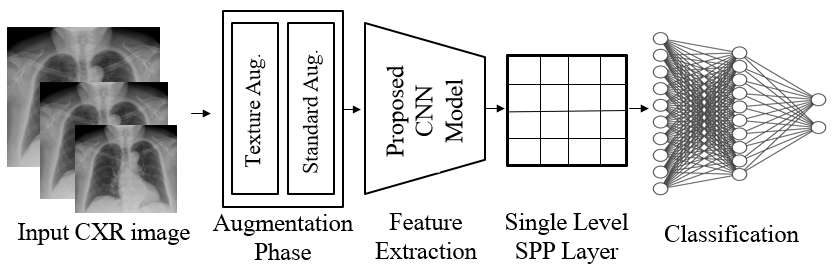
\includegraphics[height=40mm,width=15cm]{Figures/ProposedPipe.png}}
    \caption{Proposed method for COVID-19 classification from CXR images.}\label{ProposedPipe}\end{figure*}\end{center}
    
The proposed system presented in this chapter proposes a novel CNN micro-architecture model for learning scale-invariant features from row input CXR images and then classifies these features into normal or COVID-19 cases. Fig.~\ref{ProposedPipe} illustrates trainable end-to-end pipeline of the proposed system. The proposed system depends on a novel Spatially weighted Atrous Spatial Pyramid Pooling (SWASPP) to extract multi-scale features of input CXR images. A novel attention module is then used to fuse the extracted these multi-scale features and select relevant features' scale that the next layer should consider.
\subsection{Data augmentation}

\begin{center}
    \begin{figure}[htbp]
    \centerline{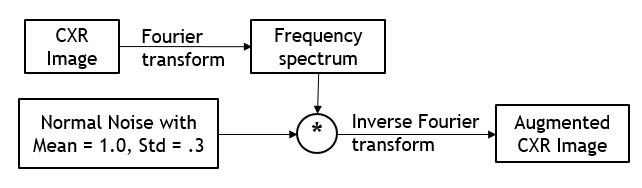
\includegraphics[height=30mm,width=9cm]{Figures/TexAug.PNG}}
    \caption{Texture Augmentation module}
    \label{texaug}
    \end{figure}
    \end{center}
The first phase of the proposed CXR classification system is data augmentation phase. Data augmentation is used to reduce the overfitting by artificially enlarge the training dataset~\cite{krizhevsky2012imagenet} using label preserving transformation. Data augmentation phase introduces a degree invariance to a distortion transformation such as the flipping and rotation. The input CXR images are augmented using texture augmentation.  Texture augmentation is performed by introducing a multiplicative normally distributed noises to the frequency spectrum of the input image. CXR image is transformed to the frequency spectrum using the fourier transform.  Noise is modeled using $\mathcal{N}(\mu = 1,\,\sigma = 0.3)$. Fig.~\ref{texaug} illustrates texture augmentation process for frequency distortion of the CXR image. Fig.~\ref{resltaug} shows the original CXR image and the corresponding frequency distorted CXR image. A standard augmentation techniques such as random rotation, horizontal flipping, and vertical flipping are included in the augmentation process. 

\begin{center}
    \begin{figure}[htbp]
    \centerline{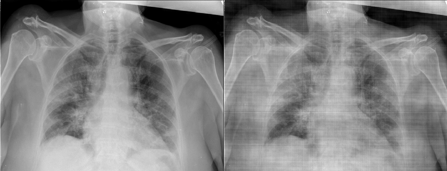
\includegraphics[height=40mm,width=9cm]{Figures/freqJitt.png}}
    \caption{Texture Augmentation}{The resulting CXR image from Texture augmentation \textbf{left}: is the original image. \textbf{Right} is the augmented  CXR Image}
    \label{resltaug}
    \end{figure}
    \end{center} 
    

\begin{center}
\begin{figure}[htbp]
\centerline{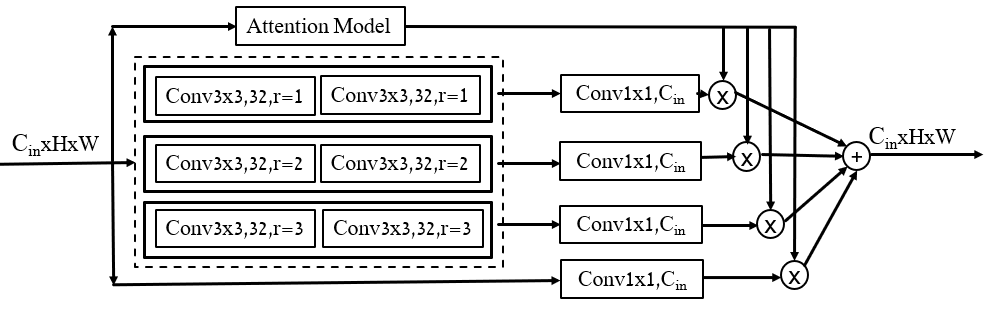
\includegraphics[height=50mm,width=9cm]{Figures/SWASPP.PNG}}
\caption{Spatially weighted atrous spatial Pyramid Pooling (SWASPP) interal layers within dashed square are parameter shared.}
\label{swaspp}
\end{figure}
\end{center}

\subsection{Spatially Weighted Atrous Spatial Pyramid Pooling}

Atrous convolution is a powerful technique for adjusting the resolution of convolutional kernels. This allows to effectively enlarge the field-of-view of the kernel without increasing neither the number of kernel parameters nor the computational complexity of the convolution operation. Atrous convolution is equivalent to performing downsampling and then performing convolution with original kernel without dilation. As a result different dilation rates of the kernel corresponding to different downsampling degrees. A novel spatially weighted atrous spatial pyramid pooling (SWASPP) micro-architecture is presented that exploit the scale space of the CNN's feature maps. Fig.~\ref{swaspp} shows the architecture of the SWASPP. In Fig.~\ref{swaspp}, internal pipelines, bounded by dashed-line square, are parameter-shared and each pipeline of these has a different dilation rates. These pipelines are responsible for extracting multi-scale, scale invariant, features. Sharing of the parameters enforce these pipelines to learn features that exists at multiple levels of scale-pyramid and hence scale-invariance. For a given input CXR image, three scales feature maps are produced.
\begin{center}
\begin{figure}[htbp]
\centerline{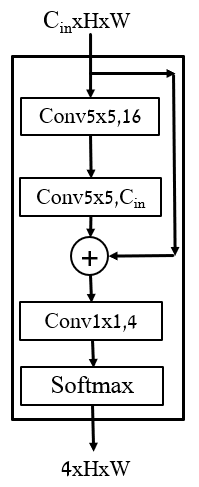
\includegraphics[height=60mm,width=3.5cm]{Figures/AttentionModUl.PNG}}
\caption{Attantion module structure used by SWASPP micro-architecture}
\label{attain}
\end{figure}
\end{center}
To fuse these feature maps produced by different pipeline of the SWASPP from the input feature map, an attention module is emerged. Attention module can be thought as a pixel level classification of which scale does this pixel it belongs to. Fig.~\ref{attain} illustrates the proposed attention module structure. Proposed attention module generates four heatmaps. The first three heatmaps correspond to the three scale feature maps while the remaining heatmap corresponds to the input feature map itself. These heatmaps are summed  up to one (\textit{i.e.,} for a  spatial position 
$(x, y)$, $\sum_{i =1}^{4} H(i,x,y) = 1$ where $H(i,x,y)$ is the $i$ heatmap produced by the attention module). To make sure this property holds, softmax function is used. 

The proposed mirco-architecture uses a pixel level weights produced by corresponding attention module rather than a single weight value for each scale. A single input CXR image may have multiple COVID-19 pneumonia scales which effectively lead to simply averaging the scale space when using single weight for each scale on scale space. In SWASPP, every convolution operation is followed by a BN and leakyReLU~\cite{krizhevsky2012imagenet} non-linearity except the re-projection layers that used to project back to the input space is not followed by nonlinearity. 
BN allows the use of larger learning rate~\cite{ioffe2015batch} and makes network stable during training~\cite{ioffe2015batch}. BN makes the loss landscape of the optimization problem significantly smoother~\cite{santurkar2018does}.
leakyReLU is used to reduce the vanishing gradient problem~\cite{krizhevsky2012imagenet}.
A bottleneck is introduced within both the attention module and multi-scale feature extractor pipeline. A bottleneck in SWASPP is used to project the input feature map of dimension $C_{in}\times H\times W$ to $32\times H\times W$ then re-project back to $C_{in}\times H\times W$. Multi-scale feature extraction is preformed on the projected dimension. Same logic is applied to the attention module where the input feature map is projected to a dimension of $16\times H\times W$.
This bottleneck allows the efficient use of model capacity and reduce the network computational complexity~\cite{huang2017densely}. It only allows the flow of important information and discarding irrelevant information. 

\subsection{Proposed CNN Architecture}
SWASPP is densely stacked~\cite{huang2017densely} together as Fig.~\ref{denseB} illustrates. This kind of connectivity allows implicit deep supervisions as each layer is effectively connected to the last layer using shorter path also facilitate feature reuse~\cite{huang2017densely} and gradient flow. Residual layers are easier to optimize if the required mapping is the identity mapping or simply near to it~\cite{he2016deep}. Densely stacked SWASPP is denoted by (DSWASPP). Convolutional part of proposed model consists of stacking six DSWASPP layers such that the first four layers are interconnected using maxpooling to reduce the spatial size and enlarge the Network receptive field. A single level Spatial Pyramid Pooling (SPP)~\cite{he2015spatial} is added after to produce a fixed size feature vector for a variable size input. SPP layer divides the input feature map into $10\times 10 = 100$ bins then performs a $max$ for each bin as an aggregation function. 
\begin{center}
\begin{figure}[htbp]
\centerline{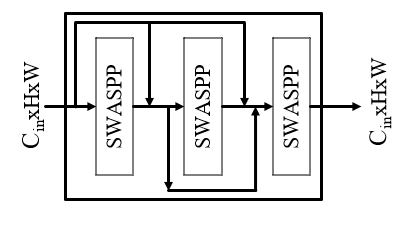
\includegraphics[height=30mm,width=6cm]{Figures/DensResd.PNG}}
\caption{Densely connected SWASPP (DSWASPP): is a stack of densely connected SWASPP, such that the output of any SWASPP is Concatenated to the input of all next layers. All the three layers produce an output of dimension of $C_{in} \times H \times W$.}
\label{denseB}
\end{figure}
\end{center}

The fixed length feature vector produced by SPP is used as an input to dropout~\cite{srivastava2014dropout} layer. Dropout layer randomly sets the activation of to $0$ with a probability of $0.5$. Dropout prevents the overfitting and reduce complex co-adaptation between the neurons allowing them to learn better representation~\cite{srivastava2014dropout}. It allow implicit ensempling of exponential number of sampled thin network from the original network which enhance the network performance~\cite{srivastava2014dropout}. The result of dropout layer is used as input to the classification network. Classification network consists of a fully connected layers with a $3$ Dense layers such that the output layer is 2-neuron for binary classification \textit{i.e)} COVID19 or not. Table~\ref{PCNN} shows the details of the proposed architecture.

\renewcommand{\arraystretch}{1.5}
\begin{table}[htbp]
    \caption{Proposed CNN architecture of methodology II}
    \begin{center}
    \begin{tabular}{|c|c|c|c|}
    \hline
    \textbf{Layer}&\multicolumn{3}{|c|}{\textbf{Proposed CNN Architecture of Methodology II}} \\
    \cline{2-4} 
    \textbf{Name} & \textbf{\textit{Input Shape}}& \textbf{\textit{Output Shape}}& \textbf{\textit{Param. Count}} \\
    \hline
    Input layer & - & $1 \times 320 \times 320$ & 0 \\
    \hline
    BatchNorm-1 & $1 \times 320 \times 320$ & $1 \times 320 \times 320$ & 2 \\
    \hline
    DSWASPP-1& $1 \times 320 \times 320$ & $32 \times 320 \times 320$ & 121,035  \\
    \hline
    Maxpooling-1& $32 \times 320 \times 320$ &$32 \times 160 \times 160$ & 0 \\
    \hline
    DSWASPP-2& $32 \times 160 \times 160$ & $64 \times 160 \times 160$ & 298,236  \\
    \hline
    Maxpooling-2 & $64 \times 160 \times 160$ & $64 \times 80 \times 80$ &0  \\
    \hline
    DSWASPP-3  & $64 \times 80 \times 80$ & $128 \times 80 \times 80$ & 604,956  \\
    \hline
    Maxpooling-3 & $128 \times 80 \times 80$ & $128 \times 40 \times 40$ & 0  \\
    \hline
    DSWASPP-4  & $128 \times 80 \times 80$ & $128 \times 80 \times 80$ & 784,092 \\
    \hline
    DSWASPP-5  & $128 \times 80 \times 80$ & $128 \times 80 \times 80$ & 784,092 \\
    \hline
    DSWASPP-6  & $128 \times 80 \times 80$ & $128 \times 80 \times 80$ & 784,092 \\
    \hline
    SPP-1 & $128 \times 80 \times 80$ & $12800$ & 0 \\
    \hline
    Dropout-1 & $12800$ & $12800$ & 0 \\
    \hline
    FC-1 & $12800$ & $128$ & 1,638,528 \\
    \hline
    FC-2 & $128$ & $128$ & 16,512 \\
    \hline
    FC-3 & $128$ & $64$ & 8,256 \\
    \hline
    FC-4 & $64$ & $2$ & 130 \\
    \hline
    Softmax & $2$ & $2$ & 0 \\
    \hline
    \hline
    \multicolumn{3}{|c|}{Total Number of Parameter}&5,040,571\\
    \hline
    \multicolumn{4}{c}{Any linear combination is followed by BN and leakyReLU nonlinearity}\\
    \multicolumn{4}{l}{excluding re-projection layer of the SWASPP modules}
    \end{tabular}
    \label{PCNN}
    \end{center}
    \end{table}

\section{Summary}

CNN is a scale variant model. Many approaches were introduced to overcome this problem such as shared networks, feature pyramid network and atrous convolution. Atrous convolution increases the receptive field of the convolutional kernel without neither increasing the parameter number nor the computational complexity. Atrous convolution is used in the proposed work II to construct the scale space of the input feature. Attention mechanism is used to guide to process the most relevant part of the feature maps. To select the correct scale and fuse multiple scales of the input feature map a spatial attention module is used. A novel CNN architecture is proposed that internally produces multiscale feature maps which is further fused using attention based mechanism. Compact representation is learned via a bottleneck dimension which is introduced in both the multiscale feature extractor module and the attention module.

 
% Chapter Template

\chapter{Experimental Results} % Main chapter title

\label{chp:results} % Change X to a consecutive number; for referencing this chapter elsewhere, use \ref{ChapterX}
In this chapter proposed methodologies are evaluated and compared with the related work.

All models are Trained using QaTa-Cov-19 \cite{ahishali2021advance} dataset using NVIDIA Tesla P-100 GPU and programmed using PyTorch.
\section{QaTa-COV19 Dataset}
\begin{center}
\begin{figure}[htbp]
\centerline{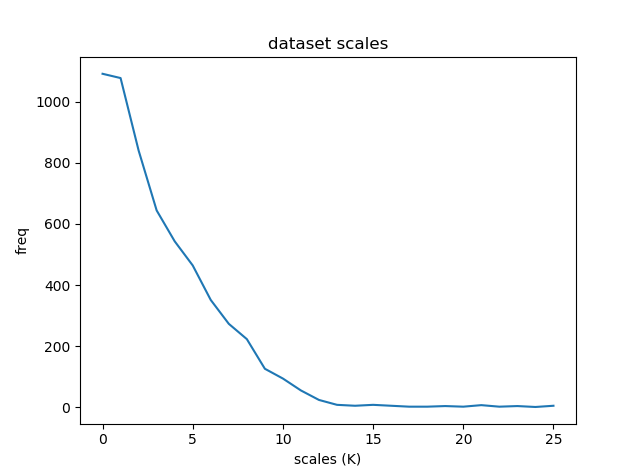
\includegraphics[height=60mm,width=9cm]{ScaleDist.png}}
\caption{Pneumonia Scales of QaTa-COV19-v1, Y-axis represents the frequency, number of occurrence, of a pneumonia with a particular area}
\label{pdist}
\end{figure}
\end{center}
QaTa-COV19 is a benchmark dataset for COVID-19 detection and Segmentation form CXR images. All models that used for comparison are trained using QaTa-COV19-v1. Qata-COV19-v1 consist of 4603 COVID-19 CXR and $120,013$ control group CXRs. A balanced number of samples for the two classes is used, namely 4603 CXR image for each class to train the models. Pneumonia Scales of QaTa-COV19-v1 does not exhibit a uniform distribution. Scale of the Pneumonia can be defined as number, area, of 8-neighbor connected pixels labeled as COVID-19 pneumonia. QaTa-COV19-v1 provides a binary masks of 2951 COVID-19 CXR image which can be used for approximating the distribution of scales across the data set. Fig. \ref{pdist} illustrates the statistical distribution of QaTa-COV19 scales. The non-uniform distribution of the scales allows the CNN models to only recognize the small scales and not large scales.

\section{Evaluation of the Methodology I}

Experiments are conducted on a Lenovo Z50-70 with Intel CORE i7-4510U CPU 2.00 GHz, 8GB RAM, NVIDIA GeForce 840M GPU; and with python and PyTorch library.

\subsection{Details of the Proposed Architecture}
The Proposed architecture composed Convbase and Densebase. Convbase is composed of a $6$ feature extraction modules \textit{(FX)} preceded by batch normalization layer as shown in Fig.5. Each FX module can be considered sub-sequential model consists of RSB layer followed by Batch Normalization, Max-pooling and LeakyReLU activation function. The Densebase is a two fully connected layers that classify the Convbase output.


\subsection{Hyperparameter Specification}
All input chest X-Ray images are resized to be $200\times 200$ . After resizing the input images, these images are fed the Convbase model part which consists of 6 layers of residual separated block. Each residual separated block is followed with batch normalization and LeakyReLU \cite{he2015delving} as activation function  as shown in. The output depth of each residual separated block is 4$\times$16, 4$\times$32, 4$\times$64, 4$\times$64, 4$\times$64 and 4$\times$16, respectively. The output of Convbase model part is 1D feature vector of 576 length. Densebase model part consists of two hidden layers. Each layer has the  size of 64 and the output layer of size 2. Each layer of Densebase layers is fully connected to its previous layer. The activation function used in the densebase model part is LeakyReLU. Table \ref{lyrSpec} summarizes the architecture hyperparameters.

\begin{table}[htbp]
\caption{The proposed architecture hyperparameters}
\begin{center}

\begin{tabular}{|l|c|c|}
\hline
\textbf{Layer Number} & \textbf{Layer Size} & \textbf{Activation Function} \\
\hline
\hline
RSBLayer1 & 4 $\times$ 16 & LeakyReLU\\
\hline
RSBLayer2 & 4 $\times$ 23 & LeakyReLU\\
\hline
RSBLayer3 & 4 $\times$ 64 & LeakyReLU\\
\hline
RSBLayer4 & 4 $\times$ 64 & LeakyReLU\\
\hline
RSBLayer5 & 4 $\times$ 64 & LeakyReLU\\
\hline
RSBLayer6 & 4 $\times$ 16 & LeakyReLU\\
\hline
\multicolumn{3}{|c|}{\textit{Flatten The Feature maps to 1D 576 feature  vector}}\\
\cline{1-3}
LinearLayer1 & 64 & LeakyReLU\\
\hline
LinearLayer2 & 64 & LeakyReLU\\
\hline
LinearLayer3 & 2 & Softmax\\
\hline
\end{tabular}
\label{lyrSpec}
\end{center}
\end{table}

\subsection{Network Training}
The proposed CNN model  is trained for 22 epoch. Adaptive Moment Estimation (Adam) optimizer \cite{kingma2014adam} is a popular optimization  technique for training deep networks. Adam optimizer is used  during the training  phase of the proposed CNN model. Both batch size and Adam optimizer learning rate is changed during the training phase if the training loss stopped decreasing. Table \ref{tabTrparam} summarizes the parameters values used in the training phase of the proposed CNN model.  Fig. \ref{fig5}(a) show the progress for training and validation loss across each epoch. The difference between the training loss and validation loss through epochs show that our did not memorize the dataset.
\begin{table}[htbp]
\caption{The change of batch size and learning rate through the Training process}
\begin{center}

\begin{tabular}{|l|c|c|}
\hline
\textbf{Epoch Number} & \textbf{Batch Size} & \textbf{Learning Rate} \\
\hline
\hline
From 0 to 6 & 128 & 1e-3\\
\hline
From 7 to 12 & 256 & 1e-3\\
\hline
From 13 to 21 & 256 & 1e-4\\
\hline
 
\end{tabular}
\label{tabTrparam}
\end{center}
\end{table}



\subsection{Model Evaluation}

To assess the efficiency of the proposed method,  the proposed method is compared to recent state-of-the-art methods for detecting Covid-19 cases. Experiments are conducted with the same dataset and the corresponding hyperparameter of each work. All the methods depend on CNN. The comparison is performed using precision, sensitivity, F1-score, and accuracy \cite{hossin2015review}. In addition, the number of the parameters used in the training phase is very important comparison factor. Table \ref{modelperf} depicts the comparison between state-of-the-art methods and the proposed method. As shown in the comparison, the proposed method  outperforms other methods achieving the maximum accuracy and the lowest  parameter count. 



\begin{table}[htbp]
\caption{ A performance comparison between the proposed method and state-of-the-art models.}
\begin{center}
\begin{tabular}{|l|c|c|c|c|c|}
\hline
\textbf{Method} & \textbf{PC} & \textbf{P(\%)}& \textbf{S(\%)}& \textbf{F1(\%)}& \textbf{A(\%)} \\
\hline
\hline
Proposed Method & 0.15M & 100.00 & 100.00 & 100.00 &100.00\\
\hline
ResNet-34 \cite{nayak2021application} & 21.8M & 96.77& 100.00 & 98.36 &98.33  \\
\hline
ACoS Phase I \cite{chandra2021coronavirus}& - & 98.266 & 96.512 & 98.551 & 98.062 \\
\hline
ResNet-50 \cite{nayak2021application}& 25.6M& 95.24& 100.00& 97.56& 97.50 \\
\hline
GoogleNet \cite{nayak2021application}& 5M &96.67& 96.67& 96.67& 96.67 \\
\hline
VGG-16 \cite{nayak2021application}& 138M& 95.08 & 96.67 & 95.87 &95.83\\
\hline
AlexNet \cite{nayak2021application}& 60M& 96.72 &98.33 & 97.52& 97.50 \\
\hline
MobileNet-V2 \cite{nayak2021application} & 3.4M &98.24& 93.33& 95.73 & 95.83 \\
\hline
Inception-V3 \cite{nayak2021application}& 24M &96.36& 88.33 & 92.17& 92.50\\
\hline
SqueezeNet \cite{nayak2021application}& 1.25M &98.27 &95.00& 96.61& 96.67 \\
\hline
\multicolumn{6}{l}{\textit{ PC is Parameter count, P is precision, S is sensitivity }}\\
\multicolumn{6}{l}{\textit{  F1 is F1-score, and A is accuracy }}\\
\hline
\end{tabular}
\label{modelperf}
\end{center}
\end{table}


\begin{figure}
\begin{center}
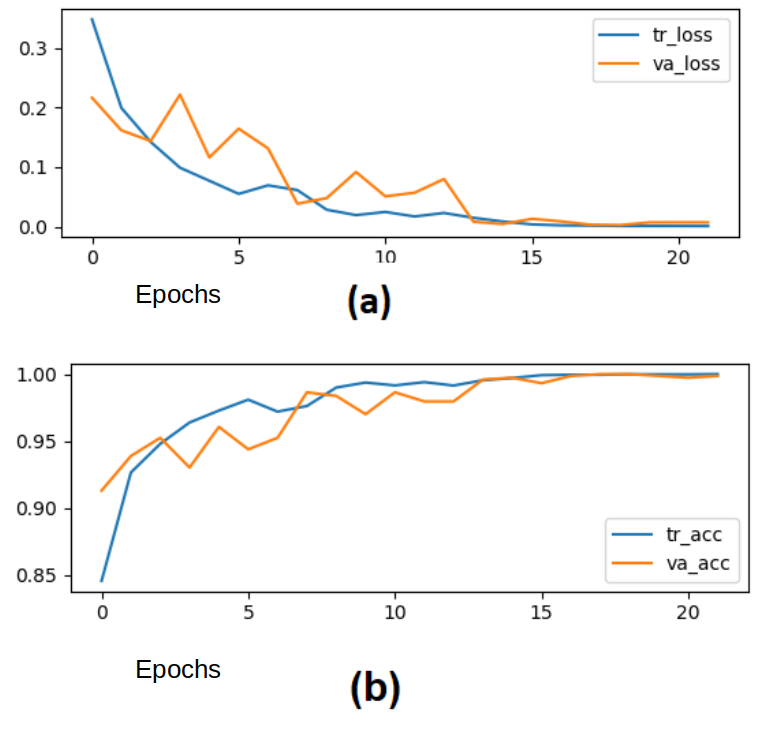
\includegraphics[height=90mm,width=8.0cm]{Figures/fig6.png}
\caption{(a) The training loss and the validation loss of each epoch and (b) The training accuracy and the validation accuracy of each epoch.}\label{fig5}\end{center}\end{figure}



\section{Evaluation of the Methodology II}
Methodology II is evaluated and compared against strong baselines and related works. 

\subsection{Baseline Networks}
Different architectures are trained to validate the effectiveness of the proposed method. 
\subsubsection{Spatial Pyramid Pooling (SPP-net) Based model}
Four variants of SPP-net\cite{he2015spatial} is trained. All $4$ variants have the same architecture but different SPP-layer. These variants of SPP-layer are as follows:
\begin{itemize}
  \item full pyramid SPP of 8-levels using average-pooling as aggregation function
  \item full SPP pyramid of 8-levels using max-pooling as aggregation function
  \item single level SPP with 10-bins using average-pooling as aggregation function
  \item single level SPP with 10-bins using max-pooling as aggregation function
\end{itemize}
  A Fixed Architecture is used for all SPP variant models with the same design principles of the proposed architecture. These architectures are the same as the proposed architecture but DSWASPP is replaced by DC6 and SPP-1 layer is replaced with the corresponding SPP layer. DC6 is defined as six convolutional layers Densely connected together. For SPP-net variants training a multiscale augmentation is added to the proposed augmentation process. Multiscale augmentation is done by randomly sampling different $5$ scales typically $\{320, 320\pm25, 320\pm50 \}$.
\subsubsection{Switchable Atrous Spatial Pyramid Pooling (SASPP-net) Based models} 
\begin{center}
\begin{figure*}[htbp]
\centerline{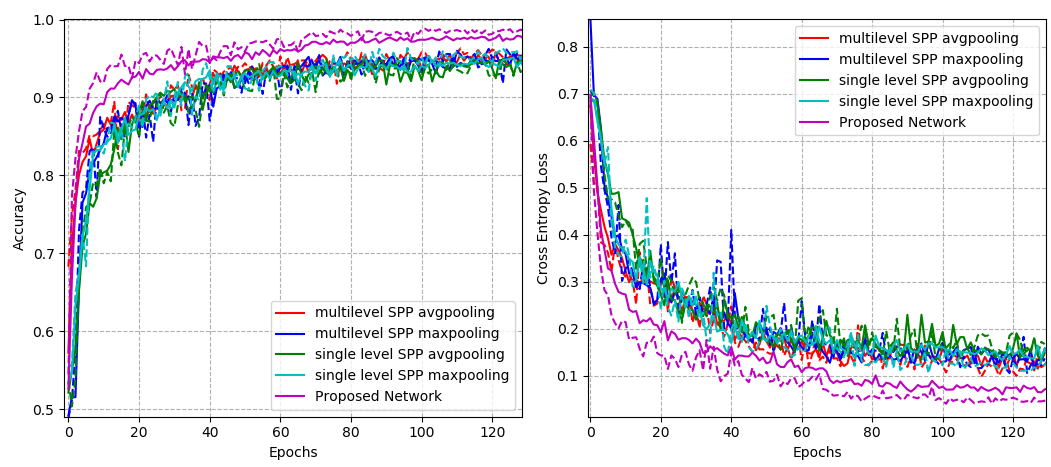
\includegraphics[height=63mm,width=15cm]{SPP-netsTraining.PNG}}
\caption{Training profiles of both SPP-net variants and the proposed network. For the same color solid line represents training statistics while dashed line represents the validation statistics for the corresponding model. \textbf{left:} is the training accuracy. \textbf{Right:} is the training loss.}
\label{SPP-train}
\end{figure*}
\end{center}

Another Base-line is introduced for comparison which is exactly as same as the proposed network but with different Attention module structure and does not include a bottleneck within ASPP. This architecture is referred Switchable Atrous Spatial Pyramid Pooling (SASPP-net). Attention module structure is $Softmax(FC(GAP(X)))$ where: \textit{$X$: is the input feature map}, \textit{$GAP$: is a global average pooling}, \textit{$FC$: is fully Connected layer performs a non-linear projection to ${\rm I\!R}^{4}$ a 4 values for the three scales and the input feature map}.\\

\begin{table}[htbp]
\caption{Baselines and their total number of parameters}
\begin{center}
\begin{tabular}{|c|c|c|}
\hline
\textbf{Model}&\multicolumn{2}{|c|}{\textbf{Baseline CNN Architectures}} \\
\cline{2-3} 
\textbf{Type} & \textbf{\textit{Variant}}& \textbf{\textit{Param. Count}} \\
\hline
  & ML Average pooling & $14,916,420$   \\
\cline{2-3} 
SPP & ML max pooling & $14,916,420$   \\
\cline{2-3} 
  & SL Average pooling & $14,490,436$   \\
\cline{2-3} 
  & SL max pooling & $14,490,436$ \\
\hline
\multicolumn{2}{|c|}{SASPP} & $13,031,841$\\
\hline
\multicolumn{3}{l}{ \textbf{ML}: Multilevel, \textbf{SL}: Single level}
\end{tabular}
\label{Basarch}
\end{center}
\end{table}
Table \ref{Basarch} summarizes the base-line models and the Corresponding parameter count.
\subsection{Models Training}
Proposed architecture and baseline architecture are trained with the same hyperparameters. Dataset is split to $0.6$, $0.2$ and $0.2$ for training, validation and testing, respectively. For training a Cross Entropy Loss is used. All models trained with ADAM \cite{kingma2014adam} optimizer with learning rate start by $10^{-3}$ and reduced every time validation loss plateau by multiplying by $10^{-1}$. A Max Norm Constraint is used to clip the gradient value to norm of $1$ \cite{krizhevsky2012imagenet}. A batch size of $128$ is used to calculate the gradient.
\subsection{Reducing the overfitting}
Overfitting is a critical problem for training large networks \cite{krizhevsky2012imagenet}. Proposed work has reduced the overfitting by using:
\begin{itemize}
\item Using Dropout with retrain probability of $0.5$ \cite{srivastava2014dropout}.
\item Using BatchNorm adds noise due to randomization introduced when constructing the minibatch \cite{ioffe2015batch}.
\item Using max norm constraint \cite{krizhevsky2012imagenet}.
\item Deep and thin architectures by design has an implicit regularization effect \cite{he2016deep}. 
\item Augmentation process i.e.) Texture augmentation \cite{krizhevsky2012imagenet}. 
\item The use of small kernel size \cite{simonyan2014very}.
\item Bottleneck in SWASPP module and the attention module.
\end{itemize}
During training no overfitting effects is observed.
\subsection{Comparison with baselines}
Proposed network is compared with the vanilla SPP-based Architectures and ASPP architecture.
\subsubsection{Comparing with SPP-nets}
Fig. \ref{SPP-train} illustrates both training loss and training and validation accuracies and losses. Table \ref{blaccom} illustrates the testing accuracy for comparison between the SPP-nets baseline and the proposed architecture.
\begin{table}[htbp]
\caption{Comparison between Proposed network and baseline SPP architectures }
\begin{center}
\begin{tabular}{|c|c|}
\hline
\textbf{Model Name}& Accurracy \\
\hline
 SPP ML Average pooling & $0.958$   \\
\hline
SPP ML max pooling & $0.950$   \\
\hline
  SPP SL Average pooling & $0.927$   \\
\hline
  SPP SL max pooling & $0.957$ \\
\hline
Proposed Network & $0.987$\\
\hline
\multicolumn{2}{l}{ \textbf{ML}: Multilevel, \textbf{SL}: Single level}
\end{tabular}
\label{blaccom}
\end{center}
\end{table}
\subsubsection{Comparing with SASPP}
Fig. \ref{saspp} illustrates the training and validation loss of training a SASPP baseline architecture. As shown in Fig. \ref{saspp} SASPP unable to generalize and start overfitting the training set. This comparison empirically shows the importance of the bottleneck introduced in the proposed architecture.

\begin{center}
\begin{figure}[htbp]
\centerline{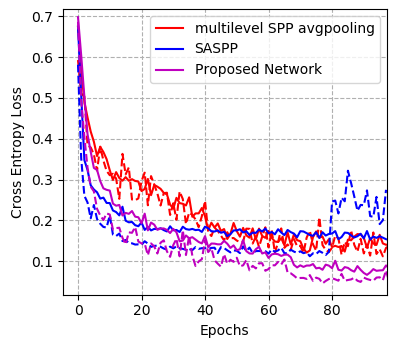
\includegraphics[height=55mm,width=8cm]{saspp.PNG}}
\caption{SASPP baseline architecture loss during both training, solid line, and validation, bashed line, compared with Proposed network and best performing SPP architecture.}
\label{saspp}
\end{figure}
\end{center}

\subsection{Comparing with the related works}
To fairly compare with the related works proposed work is further trained. Fig. \ref{ploss} shows the training and validation loss of the proposed network. Fig. \ref{pacc} shows the of the training and validation accuracy. 
\begin{center}
\begin{figure}[htbp]
\centerline{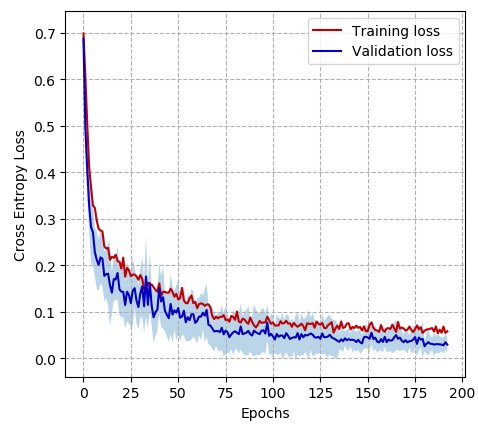
\includegraphics[height=55mm,width=8cm]{PLOSS.PNG}}
\caption{Cross entropy loss of the proposed architecture.}
\label{ploss}
\end{figure}
\end{center}
\begin{center}
\begin{figure}[htbp]
\centerline{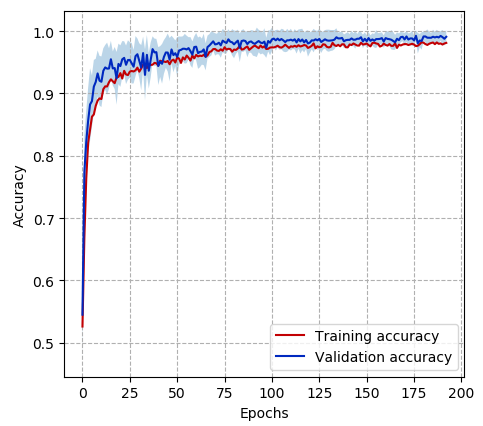
\includegraphics[height=55mm,width=8cm]{PACC.PNG}}
\caption{Training and validation accuracy of the proposed architecture.}
\label{pacc}
\end{figure}
\end{center}
Proposed Network has a sensitivity, recall, and precision of $0.994$ and $0.991$ respectively on the validation set. Precision can be improved by investigating the precision-recall trade-off. Fig. \ref{prt} shows the trade-off between precision and recall for different thresholds. A threshold of $0.618$ is used to improve the precision resulting in a sensitivity, recall, of $0.9903$ and precision of $0.9956$.
Comparison metrics are defined as follows:
\begin{itemize}
\item \textit{Accuracy}: is ratio of correctly classified samples to the total number of samples
\item \textit{Sensitivity}: is ratio of correctly classified Covid-19 samples to the total number of actual Covid-19 samples 
\item \textit{Precision}: is the ratio of correctly, according to the ground-truth labels, classified Covid-19 samples to the total number of samples classified as Covid-19.
\item \textit{Specificity}: is the ratio of correctly, according to the ground-truth labels, classified non-COVID-19 to the total number of non-Covid-19.
\item \textit{F1-score}: is the harmonic mean of both Sensitivity and Precision.
\begin{center}  
 $F_{1}=\frac{2\times\text{Precision} \times \text{Sensitivity}}{\text{Precision} + \text{Sensitivity}}$
\end{center}
\item \textit{Param. Count}: is the total number of the trainable parameters.
\end{itemize}


\begin{table*}[!p!t]
\caption{Comparison between Proposed network and Related works }
\begin{center}
\resizebox{\textwidth}{!}{\begin{tabular}{|c|c|c|c|c|c|c|}
\hline
\textbf{Model Name}& \textbf{Accuracy} & \textbf{Sensitivity} &\textbf{ Precision} & \textbf{Specificity} & \textbf{F1-score} & \textbf{Param. Count}\\
\hline
\hline
Proposed & 0.99294 & \textbf{0.9903} & \textbf{0.9956} & 0.9956 & \textbf{0.9929} & \textbf{5,040,571}\\
\hline
SRC-Dalm\cite{ar} & 0.985 & 0.886 & - & 0.993 & - & -\\
\hline 
SRC-Hom\cite{ar} & 0.977 & 0.921 & - & 0.982 & - & - \\
\hline
CRC-light\cite{ar} & 0.973 & 0.955 & - & 0.974 & - &- \\
\hline
DenseNet121*\cite{ar} & 0.992 & 0.9714 & - & 0.9949 & - & 6,955,906  \\
\hline
Inception-v3\cite{ar} & 0.993 & 0.954 & - & 0.998 & - & 21,772,450  \\
\hline
Modified MobileNetV2 \cite{akt}  & 0.98 & 0.98 & 0.97 & - & 0.97 & -\\
\hline
ReCovNet-v2\cite{dag} & 0.99726 & 0.98571 & 0.94262 & 0.9977 & 0.96369 &- \\
\hline
ReCovNet-v1\cite{dag} & 0.99824 & 0.9781 & 0.97438 & 0.99901 & 0.97624 & -\\
\hline
DenseNet-121\cite{dag}  & \textbf{0.9988} & 0.97429 & 0.9932 & \textbf{0.99974} & 0.98365 & 6,955,906 \\
\hline
\end{tabular}}
\end{center}
\label{rwcom}
\end{table*}


\begin{center}
\begin{figure}[htbp]
\centerline{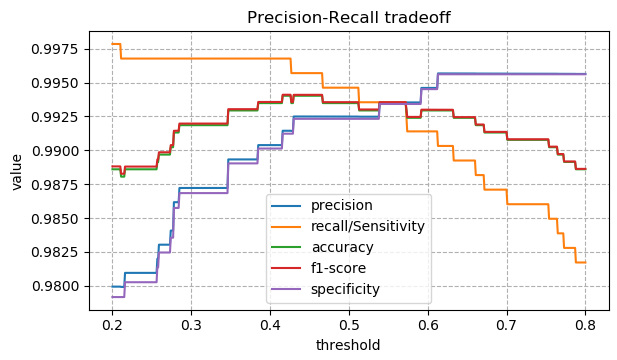
\includegraphics[height=55mm,width=8cm]{PresRecuTradff.PNG}}
\caption{precision-recall trade-off of the proposed network.}
\label{prt}
\end{figure}
\end{center}

Table \ref{rwcom} summarizes the comparison between the recent related works and the proposed architecture. Proposed architecture outperform these works in many metrics. As their training and testing does not depend on a balanced number of samples, accuracy and specificity are not good metrics for  evaluation. 


\section{Summary}
This chapter illustrates the superior performance of the proposed work I and II. Experimental results of proposed work I show the effectiveness of spatial separable kernels and residual connection for detecting COVID-19. The proposed architecture I use batch normalization to maintain the network stability during the training process. During the training process, the hyperparameters (such as batch size and learning rate) are determined dynamically. Proposed architecture I outperformed previous works for binary classification of chest X-Ray images to normal or COVID-19 cases. The proposed architecture has a very low parameter count (150K trainable parameter) compared to previous work. The proposed  architecture I achieved a performance of 100\% for accuracy, sensitivity, precision and F1-score. Proposed work I does not take care of the fact that CNN is scale variant model while proposed work II does. Better quantitative results for CXR COVID-19 classification can be obtained with a multiscale training approaches. Proposed work II internally produces multiscale feature maps using Atrous Spatial pyramid pooling. These multiscales feature maps are fused using an attention module. To learn a compact representation a bottleneck dimension is introduced in both the multiscale feature extractor module and the attention module. Proposed work II outperformed current sate-of-the-art architecture with lower parameter number. Proposed method has recorded a $0.9929$ for $F1-score$.
% Chapter Template

\chapter{Conclusion And Future Work} % Main chapter title

\label{chp:concl} % 

% COVID-19 is a severe respiratory tract infection. COVID-19 caused by SARS-CoV-2 can readily spread through contact with an infected person. Monotonically increasing SARS-CoV-2 infections have not only wasted lives but also severely damaged the financial systems of both developing and developed countries. This high spread rate pressure on the health care systems which raises the need for fast methods for diagnosing this disease. Convolutional Neural Networks (CNN) show great success for various computer vision tasks. However, CNN is a scale-variant model and is computationally expensive. In this Thesis, novel architectures are proposed for multiscale feature extraction and classification and lightweight architecture for COVID-19 diagnosing. The proposed I which is a lightweight CNN model exploits spatial kernel separability to reduce the number of the training parameters to a large extent and regularize the model to only learn linear kernel. Furthermore, This model uses residual connection and batch normalization extensively to maintain the network stability during the training process and provide the model with the regularization effect to reduce overfitting. This lightweight architecture is trained using the QaTa-Cov19 benchmark dataset achieving  100\% for accuracy, sensitivity, precision, and F1-score with a very low parameter count (150K) compared with the other methods in the literature. As a future work attention and context attention can benefit the performance. Also evaluating atrous convolution in the context of spatial separability can be beneficial. Proposed CNN II learns multiscale features using a pyramid of shared convolution kernels with different atrous rates. This scale-invariant CNN uses an attention-based mechanism that is used to guide and select the correct scale for each input. Proposed CNN II is an end-to-end trainable network and exploits a novel augmentation technique, Texture Augmentation, to reduce overfitting. Proposed method II achieved a 0.9929 for $F1-score$ tested on the QaTa-Cov19 benchmark dataset with a total of $5,040,571$ trainable parameters. SWASPP can show a great performance for the segmentation especially atrous convolution originating in the segmentation literature, Also this work can be extended to classify various pneumonia types.


\section{Conclusion}
The COVID-19 pandemic has caused severe respiratory tract infections that have rapidly spread through contact with infected individuals, resulting in devastating loss of life and economic damage worldwide. The high rate of transmission has put tremendous pressure on healthcare systems to develop fast and accurate methods for diagnosing the disease. Convolutional Neural Networks (CNNs) have shown success in various computer vision tasks, but they are scale-variant and computationally expensive. In this thesis, we proposed novel architectures for multiscale feature extraction and classification, as well as a lightweight architecture for COVID-19 diagnosis.

The proposed lightweight CNN model, referred to as CNN-I, exploits spatial kernel separability to significantly reduce the number of training parameters and regularizes the model to only learn linear kernels. To maintain network stability and reduce overfitting, residual connections, and batch normalization are extensively used. We trained this lightweight architecture on the QaTa-Cov19 benchmark dataset, achieving $100\%$ accuracy, sensitivity, precision, and F1-score with a parameter count of only 150K, which is significantly lower than other methods in the literature. As future work, attention and context attention can be explored to further enhance performance, and evaluating atrous convolution in the context of spatial separability may be beneficial.

Our second proposed architecture, CNN-II, learns multiscale features using a pyramid of shared convolution kernels with different atrous rates, making it scale-invariant. An attention-based mechanism is used to guide and select the correct scale for each input. CNN-II is an end-to-end trainable network that exploits a novel augmentation technique, Texture Augmentation, to reduce overfitting. This architecture achieved an F1-score of 0.9929 when tested on the QaTa-Cov19 benchmark dataset, with a total of 5,040,571 trainable parameters. We suggest that the SWASPP (Spatial Pyramid Atrous Spatial Pyramid Pooling) can show great performance for segmentation, especially atrous convolution originating in the segmentation literature. Additionally, this work can be extended to classify various types of pneumonia.

In conclusion, this thesis proposes novel architectures for COVID-19 diagnosis that address the limitations of traditional CNN models. These architectures achieved high accuracy while reducing computational cost and parameter count. Further research can explore attention mechanisms and evaluate the use of atrous convolution in the context of spatial separability to improve performance. This work has the potential to improve COVID-19 diagnosis and aid in the development of fast and effective methods to combat future pandemics.

\section{Suggestion for Future Work}

Further research can explore attention mechanisms and evaluate the use of atrous convolution in the context of spatial separability to improve performance. This work has the potential to improve COVID-19 diagnosis and aid in the development of fast and effective methods to combat future pandemics.




%------------
%	THESIS CONTENT - APPENDICES
%---------------

\appendix % Cue to tell LaTeX that the following "chapters" are Appendices

% Chapter Template

\chapter{\textarab[utf]{السيرة الذاتية لمقدم الرسالة} } % Main chapter title

\label{aracv} % Change X to a consecutive number; for referencing this chapter elsewhere, use \ref{ChapterX}
\begin{arab}[utf]

% \textarab[utf]{ العنوان }

\begin{itemize}
    \item \textbf{\textarab[utf]{ العنوان }}: \textarab[utf]{ سملا مركز }
\end{itemize}

\end{arab}
% Chapter Template

\chapter {\textarab[utf]{موجز الرسالة}} % Main chapter title
\label{araSummery} % Change X to a consecutive number; for referencing this chapter elsewhere, use \ref{ChapterX}
\begin{arab}[utf]

sfdsfdfsdf

\end{arab}
% Include the appendices of the thesis as separate files from the Appendices folder
% Uncomment the lines as you write the Appendices

%% Appendix A

\chapter{Frequently Asked Questions} % Main appendix title

\label{AppendixA} % For referencing this appendix elsewhere, use \ref{AppendixA}

\section{How do I change the colors of links?}

The color of links can be changed to your liking using:

{\small\verb!\hypersetup{urlcolor=red}!}, or

{\small\verb!\hypersetup{citecolor=green}!}, or

{\small\verb!\hypersetup{allcolor=blue}!}.

\noindent If you want to completely hide the links, you can use:

{\small\verb!\hypersetup{allcolors=.}!}, or even better: 

{\small\verb!\hypersetup{hidelinks}!}.

\noindent If you want to have obvious links in the PDF but not the printed text, use:

{\small\verb!\hypersetup{colorlinks=false}!}.

%\include{Appendices/AppendixB}
%\include{Appendices/AppendixC}

%---------------
%	BIBLIOGRAPHY
%---------------

\printbibliography[heading=bibintoc]

%------------

\end{document}  
